\documentclass{article}

%\usepackage[draft]{todonotes}
\usepackage{xcolor}
\usepackage[utf8]{inputenc}
\usepackage{mathtools}
\usepackage[utf8]{inputenc}
\usepackage[T1]{fontenc}
\usepackage[english]{babel}
\usepackage{graphicx}
%\usepackage{caption}
\usepackage{subcaption}
\usepackage{fixltx2e}
\usepackage{float}
\usepackage{amsthm}
\usepackage{amssymb}
\usepackage{booktabs}
\usepackage{enumitem} 
\newtheorem{definition}{Definition}
\newtheorem{theorem}{Theorem}
\usepackage{placeins}
\usepackage[a4paper, total={6in, 10in}]{geometry}


\numberwithin{equation}{subsection}
\setlength\parindent{0pt}
\setcounter{tocdepth}{2}


\begin{document}
	
	\section{Basic Logistic Growth}
	First let's take a look at the most basic case of logistic growth. The chance for the population to grow on a reproduction event is $P = 1-N_c/N_{max}$, with $N_c$ being the current population size and $N_{max}$ the maximum population size. Otherwise, the population carries on as a normal moran process.\\
	As can be seen in figure \ref{fig::NMutstime1}, the population first grows exponentially for a short while, then slows down until it stays at carrying capacity ($N_{max} = 10000$). The mutations, meanwhile, seem to behave quite differently. In the full population, the total number of mutations keeps on increasing roughly linearly for a while and starts slowing down much later than the full population. The bottleneck mutations behave very similarly, though there are obviously much fewer of them in total.\\
	In figure \ref{fig::Width1}, a simple measure for how close the distribution is to either $1/f$ or $ 1/f^2$ is shown, the ``width''. This is simply the sum of the distribution after normalizing it for the number of mutations at prevalence 1. If the tail falls of fast, the measure has a rather low value, if it falls slowly, it has a higher value. Interestingly, it appears that the full population already starts exceeding $ 1/f^2 $ even while the population is still in exponential growth (around t = 4 ), while the bottleneck population actually falls of strongly in width, even well below the $ 1/f^2 $ value.\\
	Lastly, in figure \ref{fig::VAF1}, you can see the VAF-distribution for two chosen time points. $ t = 4 $ is still in the middle of exponential growth, while $ t = 10 $ is some time after the population has reached carrying capacity. It's very notable how nice these distributions look - they can be easily drawn with a single line. Otherwise, they are mostly as expected: At $ t = 4 $, the distribution is still rather close to $ 1/f^2 $, while at $ t = 10$, the distribution already clearly starts approaching $ 1/f $. On the other hand, after the bottleneck, the distributions are both well below $1/f^2$. This is probably because the bottleneck impacts the highest frequency very strongly, so even slight initial disparaties in the highest prevalences are "carried downward", massively skewing the entire distribution.\\
	\\
	Now we look at very similar data: In figure \ref{fig::NMutstime2}, one can see again the population size vs the mutation burden of the entire population. Note that this plot is not a log-plot like the other one, to make the dynamics easier to see. Here, the maximum population size is lower ($ N_{max} = 2000$), but the dynamics at carrying capacity are continued much longer. The mutations in the full population slow down a lot, but are still increasing well after reaching carrying capacity, while the bottleneck population grows less fast initially but appears to slow down even less, comparatively.\\
	Figure \ref{fig::Width2} shows the width again for the population with $ N_{max} = 2000$. Here, we can see what happens to the bottleneck after reaching and staying at carrying capacity: It recovers tremendously from the very low width, and starts increasing towards $ 1/f $. However, while the full population has almost reached $ 1/f $, the bottleneck still has a long way to go. \\
	Figure \ref{fig::VAF2} shows the VAF for the population with $ N_{max} = 2000$, for different time points. We see basically the same as the plot for the width: The full population VAF approaches $ 1/f $ reasonably fast, with the bottleneck lagging significantly behind. Notable is how the VAF gets much less smooth over time - up to $ t = 10 $, it can still be drawn quite nicely with a line, but afterwards, it starts to go all over the place. \\
	
	\begin{figure}[h!]
		\centering
		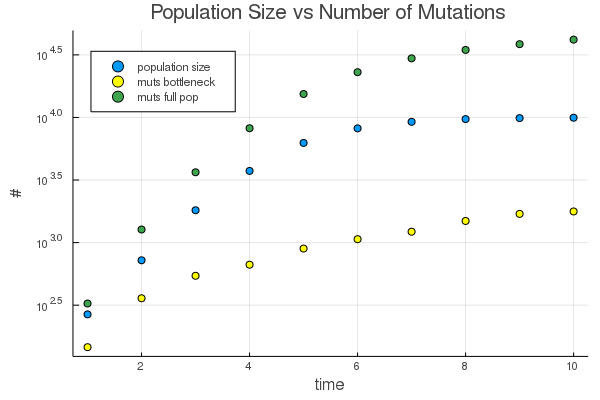
\includegraphics[width=\linewidth]{Figures/LogGrowth/document/LogGrowthBasic/LogVarTimesMutLive_N10000_mu1_t10_d1_C0}

		\caption{On the y-Axis, Population Size $N_c$ compared to the number of mutations in either the full population or the bottleneck population. On the x-Axis, time. Parameters: $ N_{max} = 10000$, $\mu = 1 $, $ S = 100 $, $ \lambda = 1$.}
		\label{fig::NMutstime1}
	\end{figure}

	\begin{figure}[h!]
		\centering
		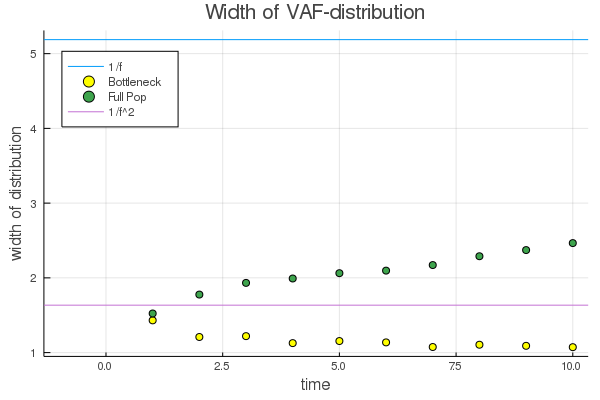
\includegraphics[width=\linewidth]{Figures/LogGrowth/document/LogGrowthBasic/LogVarTimesAlt_N10000_mu1_t10_d1_C0}
		
		\caption{On the y-Axis, width of the VAF-distribution of either the full or the bottleneck population. On the x-Axis, time. Parameters: $ N_{max} = 10000$, $\mu = 1 $, $ S = 100 $, $ \lambda = 1$.}
		\label{fig::Width1}
	\end{figure}

		\begin{figure}[h!]
		\centering
		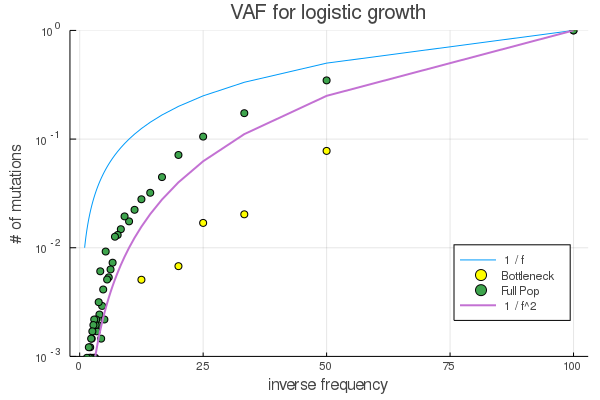
\includegraphics[width=0.49\linewidth]{Figures/LogGrowth/document/LogGrowthBasic/LogVarTimesC_N10000_mu1_t4_d1_C0}
		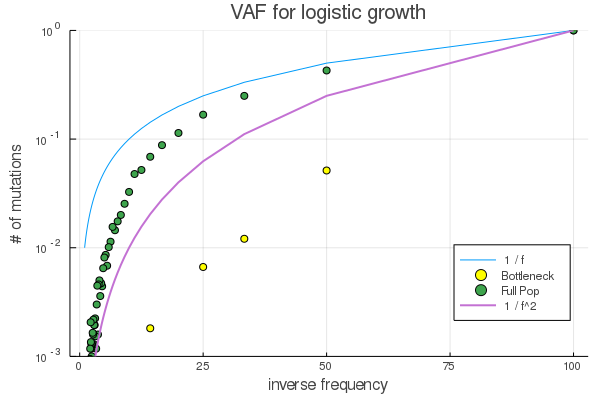
\includegraphics[width=0.49\linewidth]{Figures/LogGrowth/document/LogGrowthBasic/LogVarTimesC_N10000_mu1_t10_d1_C0}
		
		\caption{VAF-distribution. On the x-Axis, the possible prevalences for mutations. On the y-Axis, number of mutations for that prevalence in the full or the bottleneck population. . Parameters: $ N_{max} = 10000$, $\mu = 1 $, $ S = 100 $, $ \lambda = 1$. $ t =4 $ on the left, $ t= 10 $ on the right}
		\label{fig::VAF1}
	\end{figure}

		\begin{figure}[h!]
	\centering
	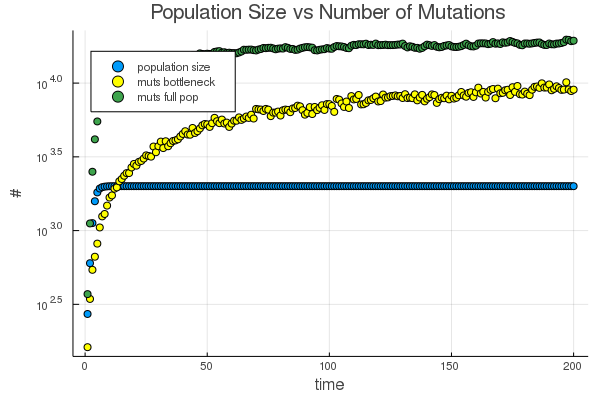
\includegraphics[width=\linewidth]{Figures/LogGrowth/document/LogGrowthBasic/LogVarTimesMutLive_N2000_mu1_t200_d1_C0}
	
	\caption{On the y-Axis, Population Size $N_c$ compared to the number of mutations in either the full population or the bottleneck population. On the x-Axis, time. Parameters: $ N_{max} = 2000$, $\mu = 1 $, $ S = 100 $, $ \lambda = 1$.}
	\label{fig::NMutstime2}
	\end{figure}
	

\begin{figure}[h!]
	\centering
	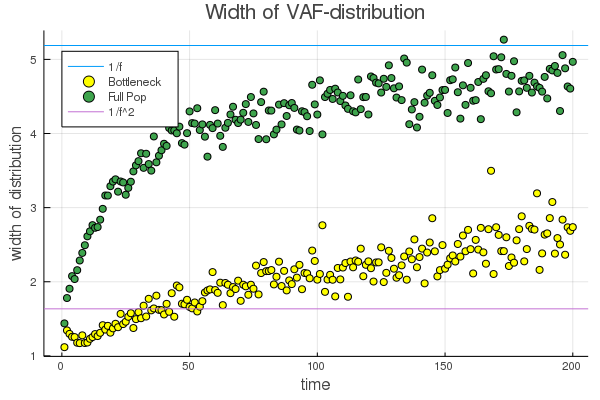
\includegraphics[width=\linewidth]{Figures/LogGrowth/document/LogGrowthBasic/LogVarTimesAlt_N2000_mu1_t200_d1_C0}
	
	\caption{On the y-Axis, width of the VAF-distribution of either the full or the bottleneck population. On the x-Axis, time. Parameters: $ N_{max} = 2000$, $\mu = 1 $, $ S = 100 $, $ \lambda = 1$.}
	\label{fig::Width2}
\end{figure}

\begin{figure}[h!]
	\centering
	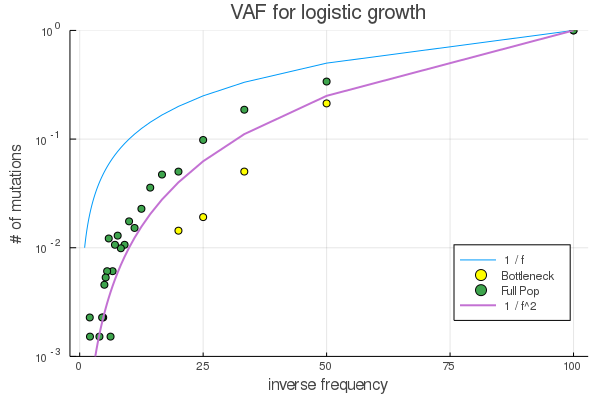
\includegraphics[width=0.49\linewidth]{Figures/LogGrowth/document/LogGrowthBasic/LogVarTimesC_N2000_mu1_t3_d1_C0}
	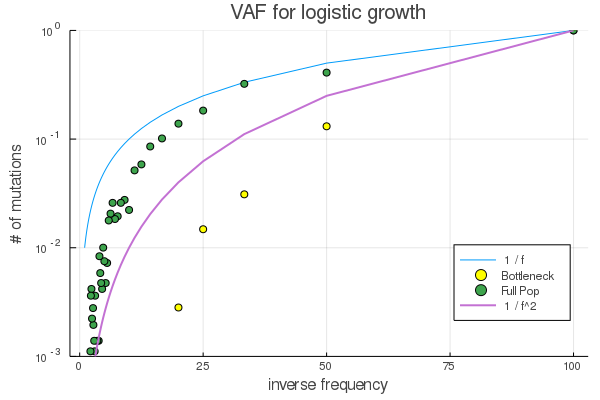
\includegraphics[width=0.49\linewidth]{Figures/LogGrowth/document/LogGrowthBasic/LogVarTimesC_N2000_mu1_t10_d1_C0}
	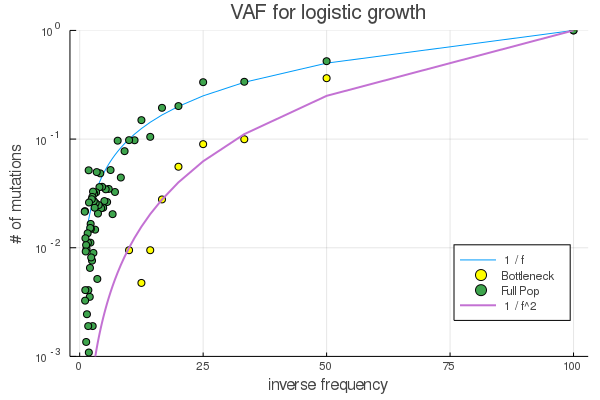
\includegraphics[width=0.49\linewidth]{Figures/LogGrowth/document/LogGrowthBasic/LogVarTimesC_N2000_mu1_t50_d1_C0}
	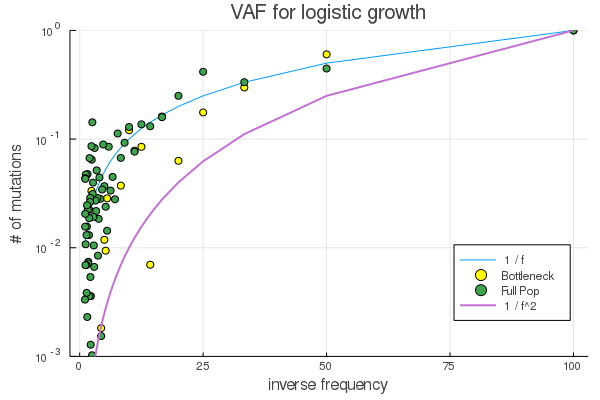
\includegraphics[width=0.49\linewidth]{Figures/LogGrowth/document/LogGrowthBasic/LogVarTimesC_N2000_mu1_t200_d1_C0}
	
	\caption{VAF-distribution. On the x-Axis, the possible prevalences for mutations. On the y-Axis, number of mutations for that prevalence in the full or the bottleneck population. . Parameters: $ N_{max} = 2000$, $\mu = 1 $, $ S = 100 $, $ \lambda = 1$. $ t =3 $ on the upper left, $ t= 10 $ on the upper right, $ t =50 $ on the lower left, $ t= 200 $ on the lower right.}
	\label{fig::VAF2}
\end{figure}
	
		
	\FloatBarrier
	
	\section{Logistic Growth - Slowdown by a fixed factor}
	
	However, what we are most interested in is what happens if we let the distribution approach 1/f relatively early, but growth happens afterwards. For this purpose, I introduced a simple factor $ d $ (for death), which modifies the chance to grow on a reproduction even : $ P_d = (1-N_c/N_{max})/d$ .So the higher the factor $ d $, the lower the chance of growing, and the more the population is dominated by moran dynamics.\\
	In figure \ref{fig::NMutstimeD}, you can see the population growth vs mutational burden again, for a rather high value of $ d = 256 $. The population is growing exponentially (it's a log-plot), and the mutations appear to grow exactly with the same speed as the population.The difference between bottleneck and full population is quite small since the full population isn't very big yet.\\
	You can see in figure \ref{fig::WidthD} the respective width of the VAF-distribution. Both the bottleneck and the full population get very close to $ 1/f $ very early, and move slightly lower over time, but still closer to $ 1/f$ than $ 1/f^2 $. The variance is unfortunately extremely high, which is also clear from figure \ref{fig::VAFD}.\\
	\\
	Now another example, with $ d = 32 $ (so much less extreme), shown in figures \ref{fig::NMutstimeD2} - \ref{fig::VAFD2}. Here, you can see how the mutations of the full population actually seem to grow in tandem with the population size, while the bottleneck grows much more slowly (though all grow exponentially). The width of the VAF reaches about halfway between $ 1/f $ and $ 1/f^2$, and the gap between the full population and the bottleneck widens again after a while. The variance in the VAF however seems a decent bit lower than the $d = 256 $ case.
	
	
	\begin{figure}[h!]
	\centering
	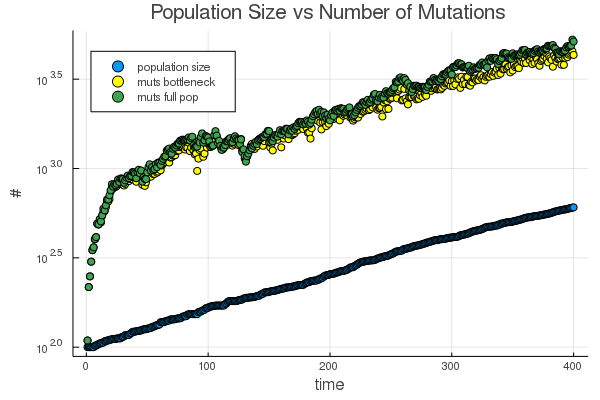
\includegraphics[width=\linewidth]{Figures/LogGrowth/document/vargrowth/LogVarTimesMutLive_N10000_mu1_t400_d256_C0}
	
	\caption{On the y-Axis, Population Size $N_c$ compared to the number of mutations in either the full population or the bottleneck population. On the x-Axis, time. Parameters: $ N_{max} = 10000$, $\mu = 1 $, $ S = 100 $, $ \lambda = 1$, $ d = 256 $.}
	\label{fig::NMutstimeD}
	\end{figure}

	\begin{figure}[h!]
	\centering
	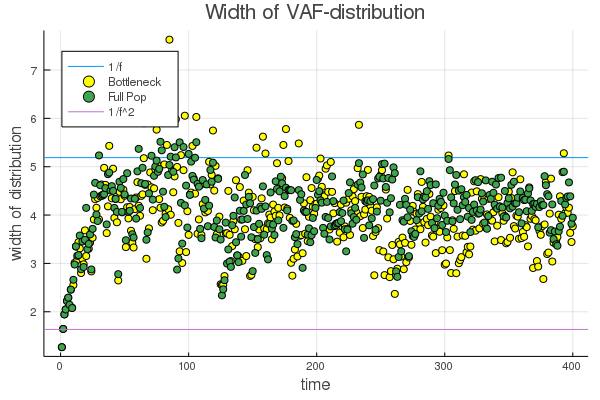
\includegraphics[width=\linewidth]{Figures/LogGrowth/document/vargrowth/LogVarTimesAlt_N10000_mu1_t400_d256_C0}
	
	\caption{On the y-Axis, width of the VAF-distribution of either the full or the bottleneck population. On the x-Axis, time. Parameters: $ N_{max} = 10000$, $\mu = 1 $, $ S = 100 $, $ \lambda = 1$, $ d = 256 $.}
	\label{fig::WidthD}
	\end{figure}

	\begin{figure}[h!]
	\centering
	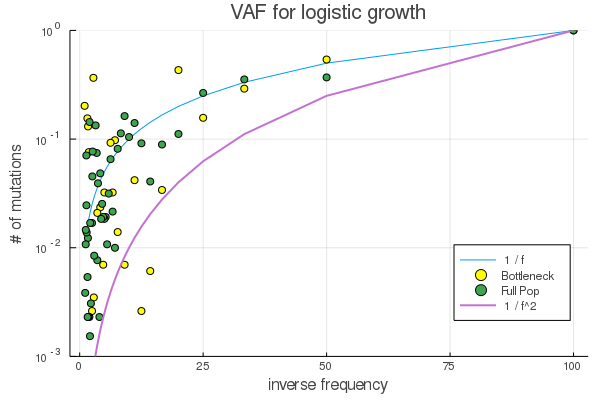
\includegraphics[width=\linewidth]{Figures/LogGrowth/document/vargrowth/LogVarTimesC_N10000_mu1_t400_d256_C0}

	
	\caption{VAF-distribution. On the x-Axis, the possible prevalences for mutations. On the y-Axis, number of mutations for that prevalence in the full or the bottleneck population. . Parameters: $ N_{max} = 1000$, $\mu = 1 $, $ S = 100 $, $ \lambda = 1$, $ d = 32 $,  $ t = 400 $.}
	\label{fig::VAFD}
	\end{figure}	
	
		\begin{figure}[h!]
		\centering
		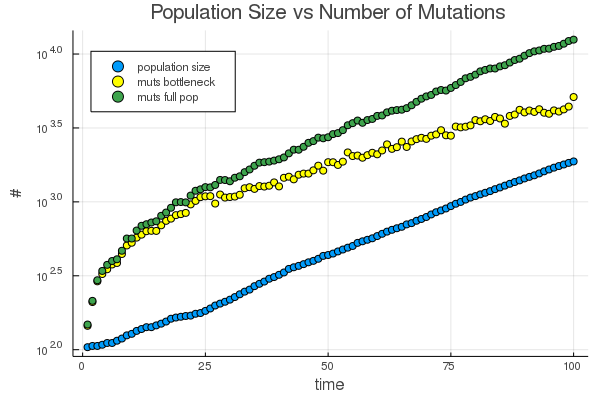
\includegraphics[width=\linewidth]{Figures/LogGrowth/document/vargrowth/LogVarTimesMutLive_N10000_mu1_t100_d32_C0}
		
		\caption{On the y-Axis, Population Size $N_c$ compared to the number of mutations in either the full population or the bottleneck population. On the x-Axis, time. Parameters: $ N_{max} = 10000$, $\mu = 1 $, $ S = 100 $, $ \lambda = 1$, $ d = 32 $.}
		\label{fig::NMutstimeD2}
	\end{figure}
	
	\begin{figure}[h!]
		\centering
		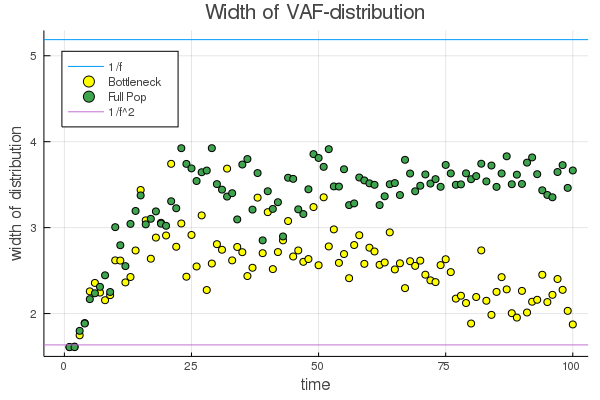
\includegraphics[width=\linewidth]{Figures/LogGrowth/document/vargrowth/LogVarTimesAlt_N10000_mu1_t100_d32_C0}
		
		\caption{On the y-Axis, width of the VAF-distribution of either the full or the bottleneck population. On the x-Axis, time. Parameters: $ N_{max} = 10000$, $\mu = 1 $, $ S = 100 $, $ \lambda = 1$, $ d = 32 $.}
		\label{fig::WidthD2}
	\end{figure}
	
	\begin{figure}[h!]
		\centering
		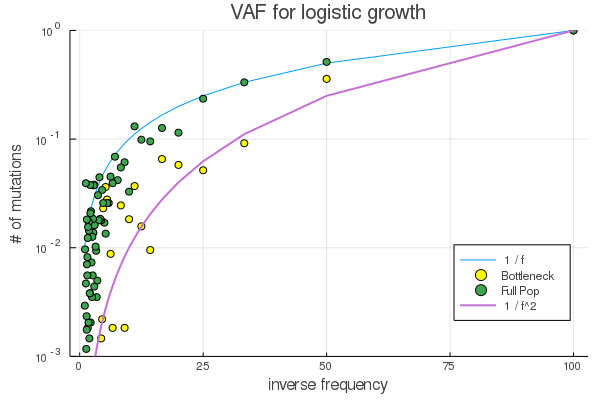
\includegraphics[width=\linewidth]{Figures/LogGrowth/document/vargrowth/LogVarTimesC_N10000_mu1_t100_d32_C0}
		
		
		\caption{VAF-distribution. On the x-Axis, the possible prevalences for mutations. On the y-Axis, number of mutations for that prevalence in the full or the bottleneck population. . Parameters: $ N_{max} = 1000$, $\mu = 1 $, $ S = 100 $, $ \lambda = 1$, $d = 32 $,  $ t = 100 $.}
		\label{fig::VAFD2}
	\end{figure}
\FloatBarrier

	\section{Logistic Growth - Stable somatic cell production}
	
	One thing Weini pointed out was that obviously, there is only limited room for an expanding population of cells. However, as Ben then answered, this is probably more true for the somatic cells then the stem cells. So I wanted to do a variant where the number of produced somatic cells is kept constant. This is simply done with a constant $ C $, which is the number of asymmetric cell divisions per unit of time. We can then calculate $ p = C/(N_c*\lambda)$, and then the simulation can be done as usual (though the check for asymmetric cell division happens before the check for a growing population, to really force the stable somatic cell production). This can have interesting effects.\\
	You can see a case with $ C = 90 $ in figures \ref{fig::NMutstimeC} - \ref{fig::VAFC}. The population only grows slowly since it is mostly just producing somatic cells initially, but it actually grows faster than exponentially afterwards because the percentage of asymmetric cell divisions go down. On the other hand, the mutational burden plateaus for quite a long time and only slowly starts increasing afterwards.
	An even more extreme case with $ C = 95$ is shown in figures \ref{fig::NMutstimeC2} - \ref{fig::VAFC2}. Again, the population grows super-exponentially, while the mutational burden is actually going down! The width plot shows us why that might happen: For basically the first 25 time points, the distribution is nothing but mutations at prevalence 1. Only somewhere around time point 50-75, the distribution approaches and surpasses $ 1/f^2$. So around that time, a large number of those low-prevalence mutations start dying out. Which is incidentally exactly the time around which the number of mutations starts going down.
	
	\begin{figure}[h!]
		\centering
		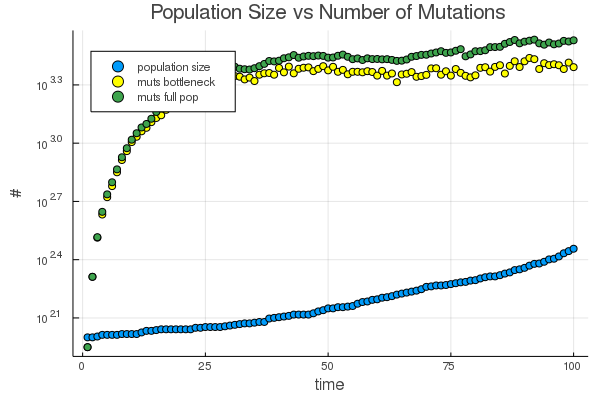
\includegraphics[width=\linewidth]{Figures/LogGrowth/document/stable_soma/LogVarTimesMutLive_N10000_mu1_t100_d32_C90}
		
		\caption{On the y-Axis, Population Size $N_c$ compared to the number of mutations in either the full population or the bottleneck population. On the x-Axis, time. Parameters: $ N_{max} = 10000$, $\mu = 1 $, $ S = 100 $, $ \lambda = 1$, $ C = 90 $.}
		\label{fig::NMutstimeC}
	\end{figure}
	
	\begin{figure}[h!]
		\centering
		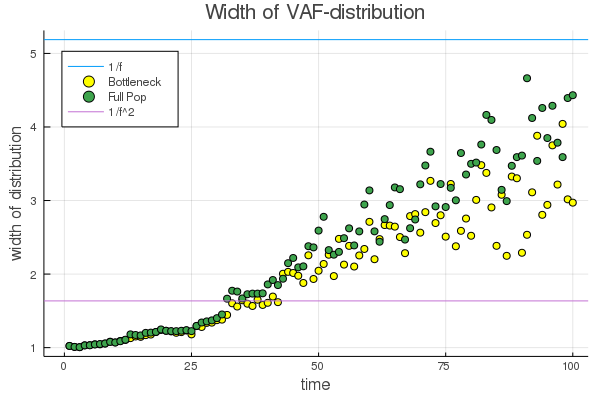
\includegraphics[width=\linewidth]{Figures/LogGrowth/document/stable_soma/LogVarTimesAlt_N10000_mu1_t100_d32_C90}
		
		\caption{On the y-Axis, width of the VAF-distribution of either the full or the bottleneck population. On the x-Axis, time. Parameters: $ N_{max} = 10000$, $\mu = 1 $, $ S = 100 $, $ \lambda = 1$, $ C = 90 $.}
		\label{fig::WidthC}
	\end{figure}
	
	\begin{figure}[h!]
		\centering
		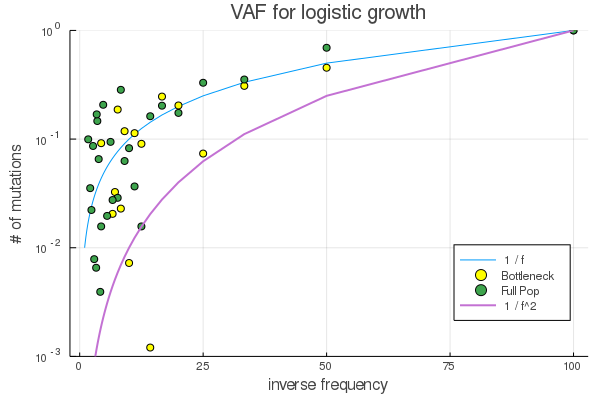
\includegraphics[width=\linewidth]{Figures/LogGrowth/document/stable_soma/LogVarTimesC_N10000_mu1_t100_d32_C90}
		
		
		\caption{VAF-distribution. On the x-Axis, the possible prevalences for mutations. On the y-Axis, number of mutations for that prevalence in the full or the bottleneck population. . Parameters: $ N_{max} = 10000$, $\mu = 1 $, $ S = 100 $, $ \lambda = 1$, $C = 90 $,  $ t = 100 $.}
		\label{fig::VAFC}
	\end{figure}

	\begin{figure}[h!]
	\centering
	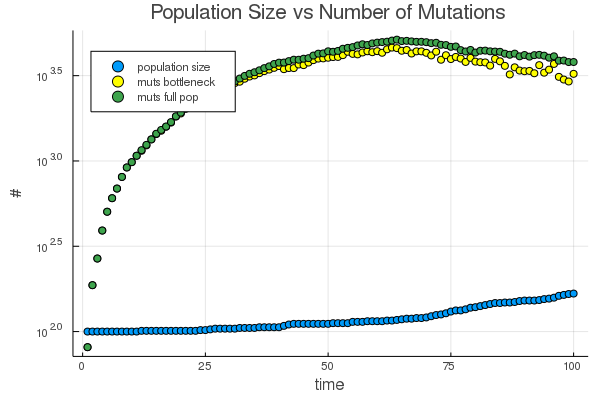
\includegraphics[width=\linewidth]{Figures/LogGrowth/document/stable_soma/LogVarTimesMutLive_N10000_mu1_t100_d32_C95}
	
	\caption{On the y-Axis, Population Size $N_c$ compared to the number of mutations in either the full population or the bottleneck population. On the x-Axis, time. Parameters: $ N_{max} = 10000$, $\mu = 1 $, $ S = 100 $, $ \lambda = 1$, $ C = 95 $.}
	\label{fig::NMutstimeC2}
\end{figure}

\begin{figure}[h!]
	\centering
	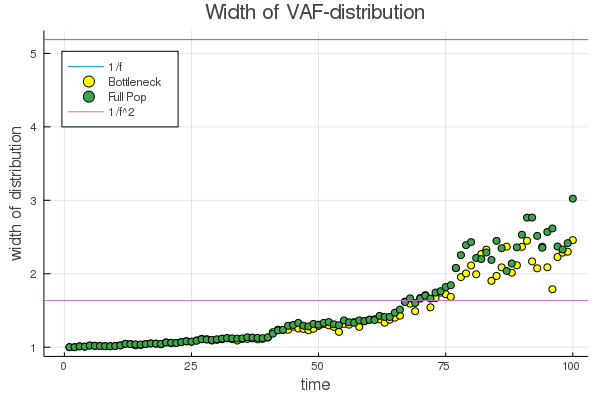
\includegraphics[width=\linewidth]{Figures/LogGrowth/document/stable_soma/LogVarTimesAlt_N10000_mu1_t100_d32_C95}
	
	\caption{On the y-Axis, width of the VAF-distribution of either the full or the bottleneck population. On the x-Axis, time. Parameters: $ N_{max} = 10000$, $\mu = 1 $, $ S = 100 $, $ \lambda = 1$, $ C = 95 $.}
	\label{fig::WidthC2}
\end{figure}

\begin{figure}[h!]
	\centering
	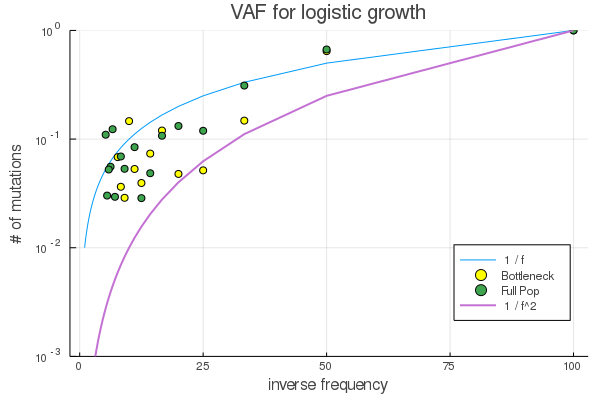
\includegraphics[width=\linewidth]{Figures/LogGrowth/document/stable_soma/LogVarTimesC_N10000_mu1_t100_d32_C95}
	
	
	\caption{VAF-distribution. On the x-Axis, the possible prevalences for mutations. On the y-Axis, number of mutations for that prevalence in the full or the bottleneck population. . Parameters: $ N_{max} = 1000$, $\mu = 1 $, $ S = 100 $, $ \lambda = 1$, $C = 95 $,  $ t = 100 $.}
	\label{fig::VAFC2}
\end{figure}
	
\end{document}